% This is file JFM2esam.tex
% first release v1.0, 20th October 1996
%       release v1.01, 29th October 1996
%       release v1.1, 25th June 1997
%       release v2.0, 27th July 2004
%       release v3.0, 16th July 2014
%   (based on JFMsampl.tex v1.3 for LaTeX2.09)
% Copyright (C) 1996, 1997, 2014 Cambridge University Press

\documentclass{jfm}
\usepackage{graphicx}
\usepackage{epstopdf, epsfig}

\newcommand{\mrd}{\mathrm{d}}
\newcommand{\cE}{\mathcal{E}}
\newtheorem{lemma}{Lemma}
\newtheorem{corollary}{Corollary}

\shorttitle{Viscous elastic fracture}
\shortauthor{T. Large, J. Lister and D. Skinner}

\title{Viscous control of shallow elastic fracture}

\author{Tim Large\aff{1},
  John Lister\aff{2},
 \and Dominic Skinner\aff{2}}
  %\corresp{\email{jfm@damtp.cam.ac.uk}}

\affiliation{\aff{1} M.I.T., USA
\aff{2}Department of Applied Mathematics and Theoretical Physics, University of
Cambridge, UK}

\begin{document}

\maketitle

\begin{abstract}
This paper considers the problem of a semi-infinite crack parallel to the
boundary of a half plane, with the crack filled by an incompressible viscous
fluid. 
The dynamics are driven by a bending moment applied to the arm of the crack,
and we look for travelling wave solutions. We examine two models of fracture;
fracture with a single tip, and fracture with a wet tip proceded by a region
of dry fracture.
\end{abstract}

\begin{keywords}
Authors should not enter keywords on the manuscript, as these must be chosen by the author during the online submission process and will then be added during the typesetting process (see http://journals.cambridge.org/data/\linebreak[3]relatedlink/jfm-\linebreak[3]keywords.pdf for the full list)
\end{keywords}

\section{Introduction}\label{sec:introduction}
Here we review the literature as well as describe the problem in more detail.
We have the vertical displacement $h$, the horizontal displacement $g$, the
thickness of the arm $l$, and the pressure $p$.
We look for a travelling wave solution (propagating left), with speed $c$.
 
\section{Formulation of problem}\label{sec:formulation_of_problem}
From lubrication, we expect Poiselle flow in the crack. This gives us the
flux, $q$, as 
\begin{equation}
q = - \frac{1}{12\mu}\frac{\mrd p}{\mrd x}h^3
\end{equation}
We also have the conservation equation
%
\begin{equation}
\frac{\partial q}{\partial x} + \frac{\partial h}{\partial t} = 0 
\end{equation}
Which combined gives us the equation
\begin{equation}
\frac{\mrd p}{\mrd x} = 12\mu c / h^2
\end{equation}
From the linear theory of elasticity, due to others who have studied this 
problem, we have
\begin{equation}
\setlength{\arraycolsep}{2pt}
\left[ \begin{array}{c} 
\sigma_y \\ \tau_{xy}
\end{array} \right]
= \int_0^{\infty} \mathsfbi{K}(\tilde{x}-x) 
\left[ \begin{array}{c} 
g'(\tilde{x}) \\ h'(\tilde{x})
\end{array} \right]
\mrd \tilde{x} 
\end{equation}
%
Where the integral kernel is
\begin{equation}
\setlength{\arraycolsep}{2pt}
\renewcommand{\arraystretch}{1.3}
\mathsfbi{K} = \left[
\begin{array}{ccccc}
  K_{11}  &  K_{12}  \\
K_{21} & K_{22} \\
\end{array}  \right] 
\end{equation}
Here we change into a set of dimensionless variables, and will spend the 
rest of the paper working with them.
We have a length scale $l$, a pressure scale $p^* = E/12(1-\nu^2)$, and a
time scale $t^* = 12\mu /p^*$.
From these, we can define the following dimensionless parameters,
\begin{equation}
\mathcal{M} = \frac{M}{p^* l^2}, \qquad \mathcal{C} = \frac{c}{l/t^*}
= \frac{12\mu c}{p^* l}, \qquad \mathcal{K}_I = \frac{K_I}{p^* l^{1/2}},
\qquad \mathcal{K}_{II} = \frac{K_{II}}{p^* l^{1/2}} 
\end{equation}
and variables 
\begin{equation} 
x = l\xi, \quad K_{ij} = U_{ij} /l, \quad h = \alpha l H(\xi), \quad
g = \alpha l G(\xi), \quad p = \beta p^* \Pi(\xi)
\end{equation}
The preferred scalings to be used in this paper are $\alpha = \upi \beta /3
= \mathcal{M}$, $\lambda = \upi\mathcal{C}/3\mathcal{M}^2$, which give
\refstepcounter{equation}
$$
\setlength{\arraycolsep}{2pt}
\left[ \begin{array}{c} 
\Pi \\ 0
\end{array} \right]
= \int_0^{\infty} \mathsfbi{U}(\tilde{\xi} - \xi) 
\left[ \begin{array}{c} 
G'(\tilde{\xi}) \\ H'(\tilde{\xi})
\end{array} \right]
\mrd \tilde{\xi}, \qquad
H^2 \frac{\mrd \Pi}{\mrd \xi} = \lambda
\eqno{(\theequation{\mathit{a},\mathit{b}})}\label{eq:govern}
$$
%
\refstepcounter{equation}
$$
\lim_{\xi \to \infty} H'' = 1 , \quad \lim_{\xi \to \infty} G' = \frac{1}{2}
\eqno{(\theequation{\mathit{a},\mathit{b}})}\label{eq:bc-at-0}
$$
%
\refstepcounter{equation}
$$
\lim_{\xi \to 0} 3\sqrt{2\pi \xi} H' = \frac{K_I}{M l^{-3/2}} \equiv \kappa_I , 
\quad
\lim_{\xi \to 0} 3\sqrt{2\pi \xi} G' = \frac{K_{II}}{M l^{-3/2}} 
\equiv \kappa_{II} , 
\eqno{(\theequation{\mathit{a},\mathit{b}})}\label{eq:by-at-inf}
$$

These shall be the governing equations for the rest of this paper, athough
we will often rewrite equation \ref{eq:govern}b as an integral, choosing
$\Pi \to 0$ as $\xi \to \infty$,
\begin{equation}\label{eq:lub-int}
\Pi(\xi) = \int_{\xi}^{\infty} \lambda / H(\tilde{\xi})^2 \mrd \tilde{\xi}
\end{equation}

Here, for completeness, we include the equations of the linear perturbation 
problem.
\begin{equation}
\Pi = \Pi_0 + \cE \Pi_1 + O(\cE), \quad
H = H_0 + \cE H_1 + O(\cE) \quad
\end{equation}
%
\refstepcounter{equation}
$$
\setlength{\arraycolsep}{2pt}
\left[ \begin{array}{c} 
\Pi_1 \\ 0
\end{array} \right]
= \int_0^{\infty} \mathsfbi{U}(\xi - \tilde{\xi}) 
\left[ \begin{array}{c} 
G_1'(\tilde{\xi}) \\ H_1'(\tilde{\xi})
\end{array} \right]
\mrd \tilde{\xi}, \qquad
H_0^2\Pi_1' + 2H_0 H_1 \Pi_0 ' = \lambda_1
\eqno{(\theequation{\mathit{a},\mathit{b}})}\label{eq:lin-pert}
$$
%
\refstepcounter{equation}
$$
H_1''\to 0 \mbox{ as\ } \xi \to \infty, \qquad
H_1 \sim \xi^{s} + \frac{\tilde{A}\lambda_1}{3\lambda_0^{2/3}} \xi^{2/3}
+ \dots \mbox{ as } \xi \to 0
\eqno{(\theequation{\mathit{a},\mathit{b}})}\label{eq:lin-pert-bc}
$$
But these can be made into a more convenient form, by considering instead
$\tilde{\Pi} = \Pi_0 - 3\lambda_0/\lambda_1 \Pi_1$, and similar for 
$\tilde{H}$, $\tilde{G}$. The equations become
\refstepcounter{equation}
$$
\setlength{\arraycolsep}{2pt}
\left[ \begin{array}{c} 
\tilde{\Pi} \\ 0
\end{array} \right]
= \int_0^{\infty} \mathsfbi{U}(\xi - \tilde{\xi}) 
\left[ \begin{array}{c} 
\tilde{G}'(\tilde{\xi}) \\ \tilde{H}'(\tilde{\xi})
\end{array} \right]
\mrd \tilde{\xi}, \qquad
H_0^2\tilde{\Pi}' + 2H_0 \tilde{H} \Pi_0 ' = 0
\eqno{(\theequation{\mathit{a},\mathit{b}})}\label{eq:rescaled-lin-pert}
$$
%
\refstepcounter{equation}
$$
\tilde{H}''\to 1 \mbox{ as\ } \xi \to \infty, \qquad
\tilde{H} \sim -\frac{3\lambda_0}{\lambda_1} \xi^{s} 
+ \dots \mbox{ as } \xi \to 0
\eqno{(\theequation{\mathit{a},\mathit{b}})}\label{eq:rescaled-lin-pert-bc}
$$
%
%
These are the equations for the two tip problem
\refstepcounter{equation}
$$
\setlength{\arraycolsep}{2pt}
\left[ \begin{array}{c} 
\Pi \\ 0
\end{array} \right]
= \int_{-L}^{\infty} \mathsfbi{U}(\tilde{\xi} - \xi) 
\left[ \begin{array}{c} 
G'(\tilde{\xi}) \\ H'(\tilde{\xi})
\end{array} \right]
\mrd \tilde{\xi}, \qquad
\Pi = \int_{\xi}^{\infty} \lambda / H(\tilde{\xi})^2 \mrd \tilde{\xi}
\eqno{(\theequation{\mathit{a},\mathit{b}})}\label{eq:2-govern}
$$
%
\refstepcounter{equation}
$$
\lim_{\xi \to \infty} H'' = 1 , \quad \lim_{\xi \to \infty} G' = \frac{1}{2}
\eqno{(\theequation{\mathit{a},\mathit{b}})}\label{eq:2-bc-inf}
$$
%
\refstepcounter{equation}
$$
\lim_{\xi \to 0} 3\sqrt{2\pi \xi} H' = 0 , 
\quad
\lim_{\xi \to -L} 3\sqrt{2\pi \xi} G' = \kappa_{II}
\eqno{(\theequation{\mathit{a},\mathit{b}})}\label{eq:2-bc-0}
$$
\section{Numerical scheme}\label{sec:numerical_scheme}
%
%
\subsection{Single Tip}
We discretize the problem by taking n points $\boldsymbol{\xi} = (\xi_1, \dots
,\xi_n)$ at which we measure $H'$, $G'$, and $n-1$ intermediate points 
$\boldsymbol{\zeta} = (\zeta_1, \dots , \zeta_{n-1})$ at which to measure
$\Pi$, so that $\xi_1 < \zeta_1 < \dots < \zeta_{n-1} < \xi_n$. We take
$\xi_1 = 0$, where the crack tip is situated.
Linear interpolation of $G'$, $H'$ would work poorly near the crack tip, since
both functions are singular there. However, both $\sqrt{\xi}G'(\xi)$, and
$\sqrt{\xi}H'(\xi)$ are regular functions, so we work with these instead.
Away from the tip, we treat $H'$, $G'$ as linear. So for 
$\xi_{i} < \xi < \xi_{i+1}$ we have that
\begin{equation}
\setlength{\arraycolsep}{2pt}
G'(\xi) = \left\{ \begin{array}{l}  
\xi^{-1/2}(a_i \xi + b_i) \\[4pt]
a_i \xi + b_i
 \end{array}\right., \quad
H'(\xi) = \left\{ \begin{array}{l}  
\xi^{-1/2}(c_i \xi^{1/2} + d_i) \\[4pt]
c_i \xi + d_i
 \end{array}\right. , \quad
\; \mbox{for\ } \left\{ \begin{array}{l}  
i<t\\[4pt]
i\geq t
\end{array}\right.
\end{equation}
Where $1 < t < n$ is just a number governing where to interpolate as linear, and
where not to; typically $t = n/2$ was used. Note that $H'$, $G$ are interpolated
slightly differently near the tip, here the choice of interpolating function 
was simply based on the appearance of $\sqrt{\xi}G'(\xi)$,$\sqrt{\xi}H'(\xi)$.
We will also define $a_n,b_n,c_n,d_n$ for interpolation beyond $\xi_n$.
We define $\boldsymbol{a} = [a_1,\dots ,a_n]$, and similarly with 
$\boldsymbol{b}$, $\boldsymbol{c}$, $\boldsymbol{d}$. We also define,
for convenience, the column vector $\boldsymbol{\gamma}=[\boldsymbol{a},
\boldsymbol{b},\boldsymbol{c},\boldsymbol{d}]$.

Now given this interpolation, suppose that we know $\boldsymbol{\gamma}$.
Then the elasticity integral (\ref{eq:govern}a), is exact; 
that is to say there is an known analytic expression for $\Pi(\xi)$, given 
our choice of interpolation.
We also have a different expression for $\Pi$, due to the lubrication integral
(\ref{eq:lub-int}).
As before, given the interpolation, the integral becomes an analytic
expression.

We see that in equation \ref{eq:govern}a, the integral depends linearly
on $\boldsymbol{\gamma}$. Therefore, we can write
\begin{equation}
[ \Pi(\zeta_{1}) , \dots , \Pi(\zeta_{n-1}), \, \underbrace{0 \, , \, \dots \, 
,\, 0 }_{n-1} \, ] = \mathsfbi{J} \boldsymbol{\gamma}
\end{equation}
where $\mathsfbi{J}$ is a matrix in lieu of the integral kernel. We also know
that $[ \Pi(\zeta_{1}) , \dots , \Pi(\zeta_{n-1})] = 
f_1( \boldsymbol{c},\boldsymbol{d})$, from the lubrication integral. This time,
$\Pi$ does not depend linearly on $\boldsymbol{\gamma}$.

We define $\boldsymbol{\theta}_G = [a_1 \xi_1 + b_1, \dots , a_n \xi_n + b_n]$,
$\boldsymbol{\theta}_H = [c_1 \xi_1^{1/2} + d_1, \dots , 
c_n \xi_n^{1/2} + d_n]$, as well as $\boldsymbol{\theta} = 
[\boldsymbol{\theta}_G, \boldsymbol{\theta}_H] $. 
We would prefer to work with $\boldsymbol{\theta}$ over $\boldsymbol{\gamma}$,
since it contains half as many elements. Continuity of $G'$, $H'$ impose 
$2(n-1)$ equations, which are typically of the form
\begin{equation}
\setlength{\arraycolsep}{1pt}
\begin{array}{rl}
a_i \xi_{i+1} + b_i~ &= a_{i+1} \xi_{i+1} + b_{i+1},\mbox{ for } i<n,
\,i\neq t -1 \\[4pt]
\xi^{-1/2}(a_i \xi_{i+1} + b_i) &= a_{i+1} \xi_{i+1} + b_{i+1},
\mbox{ for } i = t -1
\end{array}
\end{equation}
with a slightly modified equation to account for the different interpolation
in $H'$. We can also introduce some boundary conditions here to get another 
two equations. We know $G'(\xi_n)$, $G''(\xi_n)$ from our asymptotic expansion 
(via beam theory) so we know that $\theta_n = G'(\xi_n)$ and 
$a_n = G''(\xi_n)$. We can contort these relations into something linear via 
writing, 
\begin{equation}
a_n = \frac{G''(\xi_n)}{G'(\xi_n)} \theta_n, \qquad
b_n  = \theta_n - a_n \xi_n = \left( 1 - \frac{G''(\xi_n)}
{G'(\xi_n)} \right) \theta_n
\end{equation}
With $H$, we know that $a_n = H''(\xi_n)$, $a_{n-1} = H''(\xi_{n-1})$, and
so we have that 
\begin{equation}
a_n = \frac{H''(\xi_n)}{H''(\xi_{n-1})} a_{n-1}, \qquad
b_n = -a_n \xi_n + a_{n-1}\xi_n + b_{n-1}
\end{equation}
Where already we know $a_{n-1}$, $b_{n-1}$ linearly in terms of 
$\boldsymbol{\theta}$. Therefore, we have enough equations to 
calculate a matrix $\mathsfbi{T}$, so that
\begin{equation}
\boldsymbol{\gamma} = \mathsfbi{T} \boldsymbol{\theta}
\end{equation}
Although since this matrix is fairly sparse, it is 
never actually calculated in the program. To recap, we now have that
\begin{equation}
\mathsfbi{JT}\boldsymbol{\theta} = f_2(\boldsymbol{\theta}) 
\end{equation}
With $\mathsfbi{JT}$ a $2(n-1) \times 2n$ matrix, and $f_2$ a function of 
$\boldsymbol{\theta}$ (really just of $\boldsymbol{\theta}_H$), with
the first $n-1$ components calculating $\Pi$, and the last $n-1$ components
set to $0$. We add another two rows to $\mathsfbi{JT}$, to make it a square
matrix. Since we know $G'(\xi_n)$, and $H''(\xi_n) \approx 
(H'(\xi_n)-H'(\xi_{n-1}))/(\xi_n-\xi_{n-1}) = (\theta_{2n}-
\theta_{2n-1})/(\xi_n-\xi_{n-1}) $, we can replace $f_2$ with
$f = [f_2, G'(\xi_n), H''(\xi_n)]$. The two rows added have the property that
when multiplied by $\boldsymbol{\theta}$, they equal $\theta_{n}$, and
$(\theta_{2n}-\theta_{2n-1})/(\xi_n-\xi_{n-1}) $
respectively. Let the enlarged matrix be called $\mathsfbi{A}$. Then
\begin{equation}
\mathsfbi{A}\boldsymbol{\theta} = f(\boldsymbol{\theta})
\end{equation}
This can be solved by Newton's method; if $\mathsfbi{A}\boldsymbol{\theta} 
\approx f(\boldsymbol{\theta})$ and $ \mathsfbi{A}(\boldsymbol{\theta+\delta}) 
= f(\boldsymbol{\theta + \delta})$, to leading order in 
$\boldsymbol{\delta}$ we have that 
\begin{equation}
\boldsymbol{\delta} = \left(\mathsfbi{A} - D_{\boldsymbol{\theta}}f \right)^{-1}
\left( f(\boldsymbol{\theta}) - A \boldsymbol{\theta} \right)
\end{equation}
Convergence was determined to have occured when 
$\max_{\; i} |\boldsymbol{\delta}_i| < 10^{-8}$

For small values of $\lambda$, this can take two or three iterations, but as
$\lambda$ becomes closer to $\lambda_0$, it may take 10-20 iterations to 
converge.

Note that we choose a value of $\lambda$, fix the boundary conditions
at $\xi \to \infty$, then solve the problem, and subsequently recover
the boundary conditions at $\xi=0$, i.e. the $\kappa_I$, $\kappa_{II}$ values.
This can then be inverted, so that we think of $\lambda = \lambda(\kappa_I)$.
Physically, we know $\kappa_I$, and want to find $\lambda$, but in numerically
solving the problem, it makes more sense to choose $\lambda$ and recover 
$\kappa_I$.

The spacing of the points $\boldsymbol{\xi}$ makes a significant difference to 
the convergence properties. The spacing should reflect that the important 
part of the problem is happening near the tip, and this is where the points
should be concentrated. The spacing that is most often used was 
\begin{equation}
\xi_i = \tan( \chi \; i/m )^2, \quad i=1,\dots,m < n
\end{equation}
where $\chi$ is chosen so that $\tan(\chi)^2 = O(10)$, and the remaining points
are added in a geometric progression, so that 
\begin{equation}
\xi_{i+1} = (\xi_m/\xi_{m-1})\xi_{i} , \quad i = m,\dots,n-1
\end{equation}
The advantage of this, is that once one has picked an $m$, it then takes
relatively few additional points to extend out to $\xi_n \approx 800$ or so.
%
%
\subsection{Linear Perturbation Problem}
%
%
As equation \ref{eq:rescaled-lin-pert-bc}b shows, we now anticipate a 
singularity of the form $\xi^{s-1}$ in $\tilde{H}'$. We still expect a
singularity of the form $\xi^{-1/2}$ in $\tilde{G}'$. Therefore, the
interpolation used is
\begin{equation}
\setlength{\arraycolsep}{2pt}
\tilde{G}'(\xi) = \left\{ \begin{array}{l}  
\xi^{-1/2}(a_i \xi + b_i) \\[4pt]
a_i \xi + b_i
 \end{array}\right., \quad
\tilde{H}'(\xi) = \left\{ \begin{array}{l}  
\xi^{s-1}(c_i \xi + d_i) \\[4pt]
c_i \xi + d_i
 \end{array}\right. , \quad
\; \mbox{for\ } \left\{ \begin{array}{l}  
i<t\\[4pt]
i\geq t
\end{array}\right.
\end{equation}
We compute the matrices $\mathsfbi{J}$, $\mathsfbi{T}$ in a similar way as 
before (in fact many elements are exactly the same), but taking into account 
the new interpolation of $\tilde{H}'$. However, some matrix elements no longer
have a easily computable analytic expression for general $s$. In this case, 
such elements must be calculated by a numerical integration routine. 

The lubrication equation for the linear perturbation problem 
(\ref{eq:rescaled-lin-pert}b) is first transformed into an integral, where
we replace $\Pi_0'$ by  $\lambda_0 / H_0^2$ and use the boundary conditions
$\Pi_0,\Pi_1 \to 0$ as $\xi \to \infty$. We get the equation
\begin{equation}
\tilde{\Pi}(\zeta) = \int_{\zeta}^{\infty} \frac{2\lambda_0 \tilde{H}}{H_0^3} 
\mrd \xi \label{eq:lin-pert-lub}
\end{equation}
An important feature is that this is linear in $\tilde{H}$. We can integrate
each spline of $\tilde{H}'$ to get
\begin{equation}
\setlength{\arraycolsep}{2pt}
\tilde{H}'(\xi) = \left\{ \begin{array}{l}  
\xi^{s}(w_i \xi + e_i) + r_i \\[4pt]
w_i \xi^2 + e_i \xi + r_i
 \end{array}\right. , \quad
\; \mbox{for\ } \left\{ \begin{array}{l}  
i<t\\[4pt]
i\geq t
\end{array}\right.
\end{equation}
Imposing continuity at $\xi_i$ for $1< i \leq n$, and $\tilde{H}(0) =0$, there
are enough equations to obtain $\boldsymbol{w}$, $\boldsymbol{e}$, 
$\boldsymbol{r}$ linearly in terms of $\boldsymbol{c}$, $\boldsymbol{d}$.
The integrals that appear cannot be calculated analytically, so were determined 
numerically by approximating the integrand as 
\begin{equation}
\setlength{\arraycolsep}{2pt}
2\lambda_0 \tilde{H}/H_0^3 = \left\{ \begin{array}{l}  
\xi^{s-2}(p_i \xi + q_i) \\[4pt]
\xi^{-5}(p_i \xi + q_i )
 \end{array}\right. , \quad
\; \mbox{for\ } \left\{ \begin{array}{l}  
i<t\\[4pt]
i\geq t
\end{array}\right.
\end{equation}
We find $p_i$, $q_i$ by matching values at the endpoints of an interval.
Once this approximation has been made, the integrals are easily computed,
and it is straightforward to work out a formula connecting the final integral
linearly with $\boldsymbol{w}$, $\boldsymbol{e}$, $\boldsymbol{r}$.
Therefore, we end up with a matrix $\mathsfbi{R}$, such that
\begin{equation}
[ \tilde{\Pi}(\zeta_1), \dots \tilde{\Pi}(\zeta_{n-1}) ] = 
\mathsfbi{R} \boldsymbol{\theta}
\end{equation}
Padding out $\mathsfbi{R}$ with zeros, until it is of size $2n\times2n$, we
see that
\begin{equation}
\left( \mathsfbi{A} - \left[ \begin{array}{c} \mathsfbi{R} \\ \boldsymbol{0}
\end{array} \right] \right) \boldsymbol{\theta} = [0 ,\dots ,0, 
\tilde{G}'(\xi_n), \tilde{H}''(\xi_n) ] \label{eq:lin-lub-matrix}
\end{equation}
Since we haven't changed the integral kernel, the asymptotics of the kernel
remain the same, and together with the new lubrication equation, 
\ref{eq:lin-pert-lub}, we can construct an asymptotic expression for
$\tilde{H}''(\xi_n)$, $\tilde{G}'(\xi_n)$. Here, we do not need to deploy
Newton's method, as we can simply solve the linear set of equations, 
\ref{eq:lin-lub-matrix}.


\subsection{Double Tip}
In solving the problem of two tips situated at $-L$ and $0$, it is given
that $H = 0$ for $\xi <0$, and thus $H' = 0$ for $\xi <0$. We take $n$ points
to cover $0 \leq \xi < \infty$, and $r$ points to cover $-L \leq \xi < 0$.
we label these points so that
\begin{equation}
\setlength{\arraycolsep}{2pt}
\begin{array}{llllllllll}
\boldsymbol{\xi} = [ &   \xi_{1-r} = -L , & \xi_{2-r},& \dots ,& \xi_1 \quad = 0,
& \xi_2 \quad,& \dots , & \xi_t \quad,& \dots,& \xi_n \quad] \\
\boldsymbol{v} = [ &   v_{1}\quad = ~~~0 ,  & v_{2}\quad , &  \dots , 
& v_{r+1} = L , & v_{r+2}, & \dots, & v_{t+r}, & \dots, & v_{n+r} ] 
\end{array}
\end{equation}
Where $v_i = \xi_i+L$. We similarly define $\boldsymbol{\zeta}$ and 
$\boldsymbol{w}$, so that $w_i = \zeta_i+L$. It is useful to introduce a new
function $F(v) = F(L+\xi) = G(\xi)$. We interpolate $H'$ as before, and
$F'$ as,
\begin{equation}
\setlength{\arraycolsep}{10pt}
F'(v) = \left\{ \begin{array}{lcc}  
\xi^{-1/2}(a_i v + b_i) & v_i < v < v_{i+1} & i < t+r\\[4pt]
a_i \xi + b_i & v_i < v < v_{i+1} & i \geq t+r
 \end{array} \right.
\end{equation}
In the elasticity integral, the range of integration is $[-L, \infty]$. Since
$H=0$ for $\xi <0$, these limits can be replaced with $[0,\infty]$ for any
integral of $H$. We can rewrite integrals involving $G$ as
\begin{equation}
\int_{-L}^{\infty} U_{11} (\xi - \zeta) G'(\xi) \mrd \xi = 
\int_0^{\infty} U_{11}(v-(z+L)) F'(v) \mrd v =
\int_0^{\infty} U_{11}(v-w) F'(v) \mrd v
\end{equation}
Writing the equation in this way, it is clear that the numerical problem
is almost exactly the same as for the single tip problem. In fact, the 
lubrication equation \ref{eq:lub-int}, is entirely unchanged. We do not 
calculate $\Pi$ for $\xi <0$ (although it is easily done), but require that
$\sigma_{xy} = 0$ for $\xi < 0$. This provides enough equations for the problem
to be solved as before, with Newton's method. 
We input $-L$ and $\lambda$ and recover $\kappa_I$, $\kappa_{II}$, where 
$\kappa_I$ is measured at $0$. Physically, for $L>0$, we must have
$\kappa_I=0$. Numerically we solve for some $\lambda$, $L$, find $\kappa_I >0$ 
and extrapolate to $\kappa_I=0$.

The spacing of points for $\xi<0$ was chosen so that there was a concentration
of points near $-L$ and near $0$.

%
%
% 
\clearpage
\section{Results}\label{sec:Results}
%
%
%
\subsection{Single tip}
Start off with some of the basic graphs showing $H'$,$G'$, and $\Pi$ against
$\xi$.
\begin{figure}
  \centerline{\includegraphics[scale=0.3]{./../../Graphs/hprime-p-x-full.png}}
  \caption{This is a typical example of what $H'$ and $\Pi$ look like}
\end{figure}
\begin{figure}
  \centerline{\includegraphics[scale=0.3]{./../../Graphs/hprime-x.pdf}}
  \caption{This shows some evidence of the LEFM boundary layer}
\end{figure}
\begin{figure}
  \centerline{\includegraphics[scale=0.3]{./../../Graphs/pprime-x.pdf}}
  \caption{This also shows some evidence of the LEFM boundary layer}
\end{figure}
\begin{figure}
  \centerline{\includegraphics[scale=0.3]{./../../Graphs/l0.pdf}}
  \caption{Good agreement between theory and numerics here}
\end{figure}

Obvious questions to ask at this point are: How are you sure this is the right
answer, what is the effect of $n$, $t$, $\xi_{\mathrm{end}}$? Well $t$ really
doesn't have too much of an effect. This is not unexpected, in a region away
from zero, interpolating with base functions $\xi$, $1$ is similar to 
interpolating with $\xi^{-1/2}$, $\xi^{1/2}$, as both are smooth, regular 
functions. So as long as $t > O(10)$ the difference is not too noticable.
In the next graph, we determine the effect of extending $\xi_{\mathrm{end}}$,
by adding on extra points (so maintaining the same resolution near the tip).
There is a satisfactory demonstration of convergence.
\begin{figure}
  \centerline{\includegraphics[scale=0.5]{./../../Graphs/xend-march.png}}
  \caption{Satisfactory convergence as $\xi_{\mathrm{end}} \to \infty$}
\end{figure}

By adding points on in a geometric progression, it becomes quite cheap to
extend out to $\xi_{\mbox{end}} \approx 800$ or so. Once one has done this,
it is apparent that the effect of the tip resolution dominates the effect
of finite truncation, as the following figure shows.
\begin{figure}
  \centerline{\includegraphics[scale=0.3]{./../../Graphs/xend-effect-l0-D.png}}
  \caption{Shows the relatively small effect that $\xi_{\mathrm{end}}$ has
compared to the tip resolution, once $\xi_{\mathrm{end}}$ has become large
enough}
\end{figure}

By increasing $n$ (for large $\xi_{\mathrm{end}}$), we have been able to 
determine $\lambda_0$ and $D$
\begin{figure}
  \centerline{\includegraphics[scale=0.3]{./../../Graphs/l0-D.png}}
  \caption{Our best guess at $\lambda_0$ and $D$, and the approximate error
one can expect in them}
\end{figure}
\subsection{Linear perturbation problem}
We solve the linear perturbation problem. All that we really want to know
is that we see the $\xi^{s-1}$ behaviour that we expect, and we ask what the
intercept of $\tilde{H}_1$ is. It is perhaps worth mentioning the difficulties
in measuring the intercept and perhaps a notion of the sensitivity of the 
result on the estimate provided for $H_0$. Illustrating that is the next
figure 
\begin{figure}
 \centerline{\includegraphics[scale=0.3]{./../../Graphs/linear-perturbation.pdf}}
  \caption{Sensitivity of linear perturbation problem on $H_0$}
\end{figure}

Then we include the figure that shows convergence with different $n$ values
to something approaching the right answer.
\begin{figure}
 \centerline{
\includegraphics[scale=0.2]{./../../Graphs/linear-perturbation-plot.png}}
  \caption{Sensitivity of linear perturbation problem on $H_0$}
\end{figure}

\subsection{Two tips}
After the success of the linear perturbation problem, we move on to the two tip
problem. Perhaps some graphs that show an outline of the full numerical problem
with non-zero $\kappa_I$ and $\kappa_{II}$, although these are not physical.
\begin{figure}
 \centerline{
\includegraphics[scale=0.3]{./../../Graphs/KI-KII.png}}
  \caption{Visualisation of what is really a surface in 4D}
\end{figure}

What would be nice, although it doesn't exist yet, is some sort of record of
how we now extrapolate to $\kappa_I=0$. This is certainly a plot that needs to 
be made.
We now move on to the $\kappa_I=0$ set of relations.
\begin{figure}
 \centerline{
\includegraphics[scale=0.5]{./../../Graphs/KI-0.png}}
  \caption{The results of extrapolating to $\kappa_I = 0$}
\end{figure}
\section{Discussion}
This is where we discuss the figures, possibly include more figures, and draw
the results and conclusions of this paper.

Perhaps the first thing worth mentioning is the somewhat contrived, but pretty
accurate formulae for $\lambda$ in terms of $\kappa_I$. This holds for any 
toughness in the single tip case.
\begin{figure}
 \centerline{
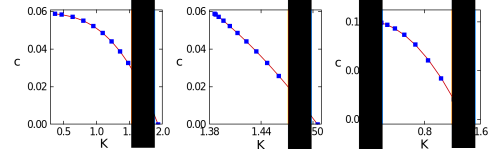
\includegraphics[scale=0.3]{./../../Graphs/overall-fit.png}}
  \caption{The formula valid for all $\kappa_I$}
\end{figure}

Then we could move on to talk about the decoupling between the fluid problem
and the dry fracture problem. Relavent graphs to include would show that
$H$ really doesn't vary much with $\lambda_0$, and that given a reference
$H'$, one can construct $G'$ with relative ease.

\begin{figure}
 \centerline{
\includegraphics[scale=0.4]{./../../Graphs/hprime-variation.png}}
  \caption{Demonstrating the decoupling of fluid and solid fracture}
\end{figure}
%
\begin{figure}
 \centerline{
\includegraphics[scale=0.4]{./../../Graphs/fixed-fluid.png}}
  \caption{Reconstructing the full solution given a reference $H'$}
\end{figure}
At this point, I would like to construct another contrived formulae for the
two tip problem. Then I would like to plot a graph of $\kappa_I$ against
$\kappa_{II}$ in the full fluid problem. This provides a guide of when it
is appropriate to take the single tip, and when it is appropriate to take
the double tip asymptotics.

\clearpage

\begin{table}
  \begin{center}
\def~{\hphantom{0}}
  \begin{tabular}{lccc}
      $a/d$  & $M=4$   &   $M=8$ & Callan \etal \\[3pt]
       0.1   & 1.56905 & ~~1.56~ & 1.56904\\
       0.3   & 1.50484 & ~~1.504 & 1.50484\\
       0.55  & 1.39128 & ~~1.391 & 1.39131\\
       0.7   & 1.32281 & ~10.322 & 1.32288\\
       0.913 & 1.34479 & 100.351 & 1.35185\\
  \end{tabular}
  \caption{Values of $kd$ at which trapped modes occur when $\rho(\theta)=a$}
  \label{tab:kd}
  \end{center}
\end{table}

\section{Citations and references}
All papers included in the References section must be cited in the article, and vice versa. Citations should be included as, for example ``It has been shown \citep{Rogallo81} that...'' (using the {\verb}\citep} command, part of the natbib package) ``recent work by \citet{Dennis85}...'' (using {\verb}\citet}).
The natbib package can be used to generate citation variations, as shown below.\\
\verb#\citet[pp. 2-4]{Hwang70}#:\\
\citet[pp. 2-4]{Hwang70} \\
\verb#\citep[p. 6]{Worster92}#:\\
\citep[p. 6]{Worster92}\\
\verb#\citep[see][]{Koch83, Lee71, Linton92}#:\\
\citep[see][]{Koch83, Lee71, Linton92}\\
\verb#\citep[see][p. 18]{Martin80}#:\\
\citep[see][p. 18]{Martin80}\\
\verb#\citep{Brownell04,Brownell07,Ursell50,Wijngaarden68,Miller91}#:\\
\citep{Brownell04,Brownell07,Ursell50,Wijngaarden68,Miller91}\\
The References section can either be built from individual \verb#\bibitem# commands, or can be built using BibTex. The BibTex files used to generate the references in this document can be found in the zip file at http://journals.cambridge.org/\linebreak[3]data/\linebreak[3]relatedlink/\linebreak[3]jfm-ifc.zip.\\
Where there are up to ten authors, all authors' names should be given in the reference list. Where there are more than ten authors, only the first name should appear, followed by et al.\\

Acknowledgements should be included at the end of the paper, before the References section or any appendicies, and should be a separate paragraph without a heading. Several anonymous individuals are thanked for contributions to these instructions.

\appendix
\section{}\label{appA}
This appendix contains sample equations in the JFM style. Please refer to the {\LaTeX} source file for examples of how to display such equations in your manuscript.

\begin{equation}
  (\nabla^2+k^2)G_s=(\nabla^2+k^2)G_a=0
  \label{Helm}
\end{equation}

\begin{equation}
  \bnabla\bcdot\boldsymbol{v} = 0,\quad \nabla^{2}P=
    \bnabla\bcdot(\boldsymbol{v}\times \boldsymbol{w}).
\end{equation}

\begin{equation}
  G_s,G_a\sim 1 / (2\upi)\ln r
  \quad \mbox{as\ }\quad r\equiv|P-Q|\rightarrow 0,
  \label{singular}
\end{equation}

\begin{equation}
\left. \begin{array}{ll}  
\displaystyle\frac{\p G_s}{\p y}=0
  \quad \mbox{on\ }\quad y=0,\\[8pt]
\displaystyle  G_a=0
  \quad \mbox{on\ }\quad y=0,
 \end{array}\right\}
  \label{symbc}
\end{equation}


\begin{equation}
  -\frac{1}{2\upi} \int_0^{\infty} \gamma^{-1}[\mathrm exp(-k\gamma|y-\eta|)
   + \mathrm exp(-k\gamma(2d-y-\eta))] \cos k(x-\xi)t\:\mathrm{d} t,
   \qquad 0<y,\quad \eta<d,
\end{equation}

\begin{equation}
  \gamma(t) = \left\{
    \begin{array}{ll}
      -\mathrm{i}(1-t^2)^{1/2}, & t\le 1 \\[2pt]
      (t^2-1)^{1/2},         & t>1.
    \end{array} \right.
\end{equation}

\[
  -\frac{1}{2\upi}
   \pvi B(t)\frac{\cosh k\gamma(d-y)}{\gamma\sinh k\gamma d}
   \cos k(x-\xi)t\:\mathrm{d} t
\]

\begin{equation}
  G = -\frac{1}{4}\mathrm{i} (H_0(kr)+H_0(kr_1))
    - \frac{1}{\upi} \pvi\frac{\mathrm{e}^{-\kgd}}%
    {\gamma\sinh\kgd} \cosh k\gamma(d-y) \cosh k\gamma(d-\eta)
\end{equation}

Note that when equations are included in definitions, it may be suitable to render them in line, rather than in the equation environment: $\boldsymbol{n}_q=(-y^{\prime}(\theta),
x^{\prime}(\theta))/w(\theta)$.
Now $G_a=\squart Y_0(kr)+\Gat$ where
$r=\{[x(\theta)-x(\psi)]^2 + [y(\theta)-y(\psi)]^2\}^{1/2}$ and $\Gat$ is
regular as $kr\ttz$. However, any fractions displayed like this, other than $\thalf$ or $\squart$, must be written on the line, and not stacked (ie 1/3).
 
\begin{eqnarray}
  \ndq\left(\frac{1}{4} Y_0(kr)\right) & \sim &
    \frac{1}{4\upi w^3(\theta)}
    [x^{\prime\prime}(\theta)y^{\prime}(\theta)-
    y^{\prime\prime}(\theta)x^{\prime}(\theta)] \nonumber\\
  & = & \frac{1}{4\upi w^3(\theta)}
    [\rho^{\prime}(\theta)\rho^{\prime\prime}(\theta)
    - \rho^2(\theta)-2\rho^{\prime 2}(\theta)]
    \quad \mbox{as\ }\quad kr\ttz . \label{inteqpt}
\end{eqnarray}

\begin{equation}
  \frac{1}{2}\phi_i = \frac{\upi}{M} \sumjm\phi_j K_{ij}^a w_j,
  \qquad i=1,\,\ldots,\,M,
\end{equation}
where
\begin{equation}
  K_{ij}^a = \left\{
    \begin{array}{ll}
      \p G_a(\theta_i,\theta_j)/\p n_q, & i\neq j \\[2pt]
      \p\Gat(\theta_i,\theta_i)/\p n_q
      + [\rho_i^{\prime}\rho_i^{\prime\prime}-\rho_i^2-2\rho_i^{\prime 2}]
      / 4\upi w_i^3, & i=j.
  \end{array} \right.
\end{equation}


\refstepcounter{equation}
$$
  \rho_l = \lim_{\zeta \rightarrow Z^-_l(x)} \rho(x,\zeta), \quad
  \rho_{u} = \lim_{\zeta \rightarrow Z^{+}_u(x)} \rho(x,\zeta)
  \eqno{(\theequation{\mathit{a},\mathit{b}})}\label{eq35}
$$

\begin{equation}
  (\rho(x,\zeta),\phi_{\zeta\zeta}(x,\zeta))=(\rho_0,N_0)
  \quad \mbox{for}\quad Z_l(x) < \zeta < Z_u(x).
\end{equation}


\begin{subeqnarray}
  \tau_{ij} & = &
    (\overline{\overline{u}_i \overline{u}_j}
    - \overline{u}_i\overline{u}_j)
    + (\overline{\overline{u}_iu^{SGS}_j
    + u^{SGS}_i\overline{u}_j})
    + \overline{u^{SGS}_iu^{SGS}_j},\\[3pt]
  \tau^\theta_j & = &
    (\overline{\overline{u}_j\overline{\theta}}
    - \overline{u}_j \overline{\theta})
    + (\overline{\overline{u}_j\theta^{SGS}
    + u^{SGS}_j \overline{\theta}})
    + \overline{u^{SGS}_j\theta^{SGS}}.
\end{subeqnarray}

\begin{equation}
\setlength{\arraycolsep}{0pt}
\renewcommand{\arraystretch}{1.3}
\slsQ_C = \left[
\begin{array}{ccccc}
  -\omega^{-2}V'_w  &  -(\alpha^t\omega)^{-1}  &  0  &  0  &  0  \\
  \displaystyle
  \frac{\beta}{\alpha\omega^2}V'_w  &  0  &  0  &  0  &  \mathrm{i}\omega^{-1} \\
  \mathrm{i}\omega^{-1}  &  0  &  0  &  0  &  0  \\
  \displaystyle
  \mathrm{i} R^{-1}_{\delta}(\alpha^t+\omega^{-1}V''_w)  &  0
    & -(\mathrm{i}\alpha^tR_\delta)^{-1}  &  0  &  0  \\
  \displaystyle
  \frac{\mathrm{i}\beta}{\alpha\omega}R^{-1}_\delta V''_w  &  0  &  0
    &  0  & 0 \\
  (\mathrm{i}\alpha^t)^{-1}V'_w  &  (3R^{-1}_{\delta}+c^t(\mathrm{i}\alpha^t)^{-1})
    &  0  &  -(\alpha^t)^{-2}R^{-1}_{\delta}  &  0  \\
\end{array}  \right] .
\label{defQc}
\end{equation}

\begin{equation}
\etb^t = \skew2\hat{\etb}^t \exp [\mathrm{i} (\alpha^tx^t_1-\omega t)],
\end{equation}
where $\skew2\hat{\etb}^t=\boldsymbol{b}\exp (\mathrm{i}\gamma x^t_3)$. 
\begin{equation}
\mbox{Det}[\rho\omega^2\delta_{ps}-C^t_{pqrs}k^t_qk^t_r]=0,
\end{equation}

\begin{equation}
 \langle k^t_1,k^t_2,k^t_3\rangle = \langle
\alpha^t,0,\gamma\rangle  
\end{equation}

\begin{equation}
\boldsymbol{f}(\theta,\psi) = (g(\psi)\cos \theta,g(\psi) \sin \theta,f(\psi)).
\label{eq41}
\end{equation}

\begin{eqnarray}
f(\psi_1) = \frac{3b}{\upi[2(a+b \cos \psi_1)]^{{3}/{2}}}
  \int^{2\upi}_0 \frac{(\sin \psi_1 - \sin \psi)(a+b \cos \psi)^{1/2}}%
  {[1 - \cos (\psi_1 - \psi)](2+\alpha)^{1/2}}\mathrm{d}x,
\label{eq42}
\end{eqnarray}
\begin{eqnarray}
g(\psi_1) & = & \frac{3}{\upi[2(a+b \cos \psi_1)]^{{3}/{2}}}
  \int^{2\upi}_0 \left(\frac{a+b \cos \psi}{2+\alpha}\right)^{1/2}
  \left\{ \astrut f(\psi)[(\cos \psi_1 - b \beta_1)S + \beta_1P]
  \right. \nonumber\\
&& \mbox{}\times \frac{\sin \psi_1 - \sin \psi}{1-\cos(\psi_1 - \psi)}
  + g(\psi) \left[\left(2+\alpha - \frac{(\sin \psi_1 - \sin \psi)^2}
  {1- \cos (\psi - \psi_1)} - b^2 \gamma \right) S \right.\nonumber\\
&& \left.\left.\mbox{} + \left( b^2 \cos \psi_1\gamma -
  \frac{a}{b}\alpha \right) F(\frac{1}{2}\upi, \delta) - (2+\alpha)
  \cos\psi_1 E(\frac{1}{2}\upi, \delta)\right] \astrut\right\} \mathrm{d} \psi,
\label{eq43}
\end{eqnarray}
\begin{equation}
\alpha = \alpha(\psi,\psi_1) = \frac{b^2[1-\cos(\psi-\psi_1)]}%
  {(a+b\cos\psi) (a+b\cos\psi_1)},
  \quad
  \beta - \beta(\psi,\psi_1) = \frac{1-\cos(\psi-\psi_1)}{a+b\cos\psi}.
\end{equation}


\begin{equation}
\left. \begin{array}{l}
\displaystyle
H(0) = \frac{\epsilon \overline{C}_v}{\tilde{v}^{{1}/{2}}_T
(1- \beta)},\quad H'(0) = -1+\epsilon^{{2}/{3}} \overline{C}_u
+ \epsilon \skew5\hat{C}_u'; \\[16pt]
\displaystyle
H''(0) = \frac{\epsilon u^2_{\ast}}{\tilde{v}^{{1}/{2}}
_T u^2_P},\quad H' (\infty) = 0.
\end{array} \right\}
\end{equation}

\begin{lemma}
Let $f(z)$ be a trial \citet[][pp.~231--232]{Batchelor59} function defined on $[0,1]$.  Let $\varLambda_1$ denote
the ground-state eigenvalue for $-\mathrm{d}^2g/\mathrm{d} z^2=\varLambda g$,
where $g$ must satisfy $\pm\mathrm{d} g/\mathrm{d} z+\alpha g=0$ at $z=0,1$
for some non-negative constant~$\alpha$.  Then for any $f$ that is not
identically zero we have
\begin{equation}
\frac{\displaystyle
  \alpha(f^2(0)+f^2(1)) + \int_0^1 \left(
  \frac{\mathrm{d} f}{\mathrm{d} z} \right)^2 \mathrm{d} z}%
  {\displaystyle \int_0^1 f^2\mathrm{d} z}
\ge \varLambda_1 \ge
\left( \frac{-\alpha+(\alpha^2+8\upi^2\alpha)^{1/2}}{4\upi} \right)^2.
\end{equation}
\end{lemma}

\begin{corollary}
Any non-zero trial function $f$ which satisfies the boundary condition
$f(0)=f(1)=0$ always satisfies
\begin{equation}
  \int_0^1 \left( \frac{\mathrm{d} f}{\mathrm{d} z} \right)^2 \mathrm{d} z.
\end{equation}
\end{corollary}

\bibliographystyle{jfm}
% Note the spaces between the initials
\bibliography{elastic-fracture}

\end{document}
